\documentclass[12pt]{article}
\usepackage[margin=0.7in]{geometry}
\usepackage{amsmath}
\usepackage{hyperref}
\usepackage{graphicx}
\usepackage{float}
\usepackage{caption}
\usepackage{subcaption}
\usepackage{listings}

\title{Numerical Algorithms: Assignment 13}
\author{Niccolo Zuppichini}
\begin{document}

\maketitle
\begin{equation}
\Phi_{E}=\frac{Q}{\varepsilon_{0}}
\end{equation}
\section*{Exercise 1}

The function is odd (i.e. $f(-x) = -f(x)$) therefore all the cosine terms $a_k$ are zero. The Fourier of expansion of $f(x)$ is then:

\begin{equation}
	f(x) = \sum_{k=1}^{\infty} b_k sin(kx)
\end{equation}

To compute the coefficients $b_k$ we need to solve: 

\begin{equation}
	b_k = \frac{1}{\pi} \int_{- \pi}^{\pi} f(x) sin(kx) dx \quad \texrm{for} \; k \geq 1
\end{equation}

To solve this integral I have used an "iterative" generalisation of integral by parts:

\begin{equation}
	\int u v dx = u v_1 - u' v_2 + u'' v_3 - u''' v_4 + ...
\end{equation}

with $u', u'', ...$ and $v_1, v_2, ...$ are successive derivatives of $u$ and integrals of $v$.  Choosing $u = f(x)$ and $v = sin(kx)$ yields: \\

\begin{equation}
	b_k = \frac{1}{\pi} \bigg[ 
	x^3 \big(\frac{-cos(kx)}{k} \big) 
	-3x^2 \big( \frac{-sin(kx)}{k^2} \big) 
	+ 6x \big( \frac{cos(kx)}{k^3} \big)
	- 6 \big( \frac{sin(kx)}{k^4} \big) 
	\bigg]_{- \pi}^{\pi} =
\end{equation}

We notice that $sin(k \pi) = sin(-k \pi) = 0$. 

\begin{equation}
\begin{split}
	= \frac{1}{\pi} \bigg[ 
	x^3 \big(\frac{-cos(kx)}{k} \big) 
	+ 6x \big( \frac{cos(kx)}{k^3} \big)
	\bigg]_{- \pi}^{\pi} &=  \\
	= \frac{1}{\pi} \bigg( 
	\pi^3 \big(\frac{-cos(k \pi)}{k} \big)
	- (-\pi)^3 \big(\frac{-cos(k (-\pi))}{k} \big) 
	+ 6\pi \big( \frac{cos(\pi x)}{k^3} \big)
	- 6(-\pi) \big( \frac{cos(- \pi x)}{k^3} \big)
	\bigg) &=
\end{split}
\end{equation}
	
By rearranging the equation and recalling that cosine is an even function (i.e. $f(x) = f(-x)$) it follows

\begin{equation}
	= \frac{1}{\pi} \bigg( 
	-2 \pi^3 \frac{cos(k \pi)}{k}  
	+ 12\pi \big( \frac{cos(\pi x)}{k^3} \big)
	\bigg) =
	2  cos(k \pi) \big( 
	- \frac{\pi^2}{k}  
	+ \frac{6}{k^3} 
	\big) =
\end{equation}

We notice that $cos(k \pi) = -1^k$

\begin{equation}
	= 2  (-1)^k \big( 
	\frac{6}{k^3} 
	- \frac{\pi^2}{k}  
	\big)
\end{equation}

Therefore the Fourier expansion of $f(x)$ is

\begin{equation}
		f(x) = \sum_{k=1}^{\infty} 2  (-1)^k \big( 
	\frac{6}{k^3} 
	- \frac{\pi^2}{k}  
	\big)
	 sin(kx)
\end{equation}

\section*{Exercise 2}

The code has been implemented in \textit{exercise2.py} using Python 3. It was not specified what the code should return as output. I thought it was interesting (and easier to visualise) to plot the real and imaginary components of the Fourier coefficients(Fig.\ref{fig:result}). The imaginary part is close to zero, but not zero. The same results are reported in Lst. \ref{lst:result}

\begin{figure}[H]
	\centering
	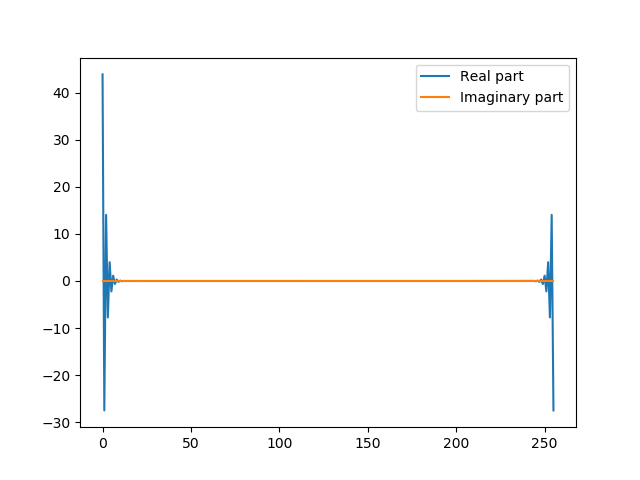
\includegraphics[width=0.7 \linewidth]{plot}
	\caption{The real and imaginary components}
	\label{fig:result}
\end{figure}



\begin{lstlisting}[caption=Results in vector form, label=lst:result]
[ 4.39487644e+01+0.00000000e+00j -2.75285556e+01-1.69309011e-15j
  1.40598970e+01+9.71445147e-16j -7.75257338e+00-9.36750677e-16j
  4.00104568e+00+2.08166817e-16j -2.21830159e+00+2.63677968e-16j
  1.12639365e+00+3.15719673e-16j -6.42237697e-01+1.73472348e-18j
  3.11321361e-01+1.38777878e-17j -1.90623565e-01+2.02095285e-16j
  8.19431099e-02-1.30971622e-16j -5.99608818e-02+1.79543880e-16j
  1.83897270e-02-1.39862080e-17j -2.13634396e-02-2.25514052e-17j
  1.45856134e-03-3.38000027e-16j -9.42091295e-03+7.60520390e-16j
 -2.56092214e-03-8.13151629e-20j -5.34887253e-03+2.88363897e-16j
 -3.13347079e-03-1.33289105e-16j -3.70108669e-03+2.01986865e-16j
 -2.87526258e-03-2.50450702e-17j -2.86687432e-03+1.30619257e-16j
 -2.48310609e-03-5.80048162e-17j -2.34984465e-03+1.20996962e-16j
 -2.12488230e-03-1.49077799e-18j -1.98412550e-03+2.77189838e-16j
 -1.82834327e-03-8.05833265e-17j -1.70607737e-03+1.54444599e-16j
 -1.58781412e-03-5.91330641e-17j -1.48630091e-03+4.79081835e-17j
 -1.39223577e-03-4.80706444e-16j -1.30848070e-03+6.44470312e-16j
 -1.23173460e-03-5.42101086e-20j -1.16225162e-03-1.03036476e-15j
 -1.09860957e-03-4.23092957e-18j -1.04046339e-03+7.89468588e-17j
 -9.87045902e-04-8.45000068e-18j -9.37943036e-04-5.23805175e-17j
 -8.92660153e-04-2.10064171e-16j -8.50836904e-04+2.09738910e-16j
 -8.12118981e-04-7.96888597e-18j -7.76215219e-04+2.32073475e-16j
 -7.42857690e-04+6.74509277e-17j -7.11815092e-04+2.18548053e-16j
 -6.82878945e-04+1.58022467e-17j -6.55865332e-04-3.17413739e-16j
 -6.30609199e-04+5.03747434e-17j -6.06963330e-04+7.04799175e-17j
 -5.84795422e-04+6.09863722e-20j -5.63986664e-04+3.39416266e-16j
 -5.44429930e-04+2.94482863e-16j -5.26028532e-04-5.56805578e-17j
 -5.08694970e-04+1.31866089e-17j -4.92349930e-04+3.72254040e-17j
 -4.76921374e-04-3.02966745e-17j -4.62343758e-04-2.72043266e-16j
 -4.48557340e-04-2.37694386e-17j -4.35507581e-04-3.28552222e-16j
 -4.23144607e-04-1.07183549e-16j -4.11422741e-04+1.89715051e-16j
 -4.00300088e-04-3.93543366e-16j -3.89738167e-04-1.17886234e-16j
 -3.79701582e-04-8.40355469e-16j -3.70157735e-04-4.95560464e-16j
 -3.61076559e-04+0.00000000e+00j -3.52430295e-04+7.25418445e-16j
 -3.44193280e-04+4.34833046e-16j -3.36341759e-04+3.31111955e-16j
 -3.28853725e-04-2.69995987e-17j -3.21708761e-04+1.65246811e-16j
 -3.14887911e-04-1.96631922e-16j -3.08373555e-04-1.60956589e-16j
 -3.02149298e-04-9.20386000e-18j -2.96199875e-04+3.40032906e-17j
 -2.90511055e-04-1.26401033e-16j -2.85069562e-04+2.00238589e-16j
 -2.79863002e-04-8.53809211e-18j -2.74879791e-04-4.22161221e-18j
 -2.70109098e-04+1.74624312e-17j -2.65540786e-04+2.34079249e-16j
 -2.61165361e-04+3.38813179e-20j -2.56973928e-04-2.39900059e-16j
 -2.52958143e-04-2.00983978e-17j -2.49110177e-04+1.30565047e-16j
 -2.45422682e-04-2.96935870e-17j -2.41888753e-04+2.55505794e-16j
 -2.38501901e-04-2.28224557e-17j -2.35256024e-04+2.24375640e-16j
 -2.32145383e-04-5.74627151e-18j -2.29164576e-04+1.53401055e-16j
 -2.26308518e-04+1.71032893e-17j -2.23572419e-04+5.08219768e-17j
 -2.20951768e-04-5.72289340e-17j -2.18442314e-04+2.24768663e-16j
 -2.16040051e-04-7.56314025e-16j -2.13741203e-04+1.64460573e-15j
 -2.11542211e-04+5.42101086e-20j -2.09439720e-04+1.83704506e-17j
 -2.07430567e-04-3.20921302e-16j -2.05511771e-04+1.05719876e-16j
 -2.03680524e-04+2.73693286e-17j -2.01934178e-04+1.40471944e-16j
 -2.00270240e-04-1.12079400e-16j -1.98686366e-04+4.05030827e-16j
 -1.97180345e-04-6.50521303e-19j -1.95750103e-04-1.76182853e-18j
 -1.94393688e-04-1.00126071e-16j -1.93109270e-04-9.28890211e-17j
 -1.91895131e-04+3.88144378e-17j -1.90749664e-04-1.47993597e-17j
 -1.89671366e-04+5.05780313e-17j -1.88658833e-04+9.36256010e-16j
 -1.87710759e-04+1.35525272e-19j -1.86825929e-04-2.59740959e-16j
 -1.86003217e-04-8.07866144e-17j -1.85241585e-04-2.79724161e-17j
 -1.84540076e-04-1.62630326e-17j -1.83897814e-04+1.66533454e-16j
 -1.83314004e-04-7.28583860e-17j -1.82787922e-04+1.07552856e-16j
 -1.82318923e-04-5.20417043e-17j -1.81906433e-04-2.00360561e-16j
 -1.81549947e-04-8.32667268e-17j -1.81249032e-04+1.73472348e-16j
 -1.81003324e-04-5.41233725e-16j -1.80812524e-04+1.24900090e-15j
 -1.80676403e-04+3.60822483e-16j -1.80594796e-04+4.16333634e-16j
 -1.80567604e-04+0.00000000e+00j -1.80594796e-04+1.94289029e-16j
 -1.80676403e-04-1.38777878e-16j -1.80812524e-04+1.73472348e-16j
 -1.81003324e-04-1.38777878e-17j -1.81249032e-04-6.93889390e-17j
 -1.81549947e-04+3.81639165e-17j -1.81906433e-04+2.09901541e-16j
 -1.82318923e-04-6.93889390e-18j -1.82787922e-04+2.02095285e-16j
 -1.83314004e-04-1.03216047e-16j -1.83897814e-04+8.58688121e-17j
 -1.84540076e-04-6.25584654e-17j -1.85241585e-04+1.05818132e-16j
 -1.86003217e-04+1.00126071e-16j -1.86825929e-04+5.32404253e-16j
 -1.87710759e-04+2.71050543e-20j -1.88658833e-04+6.44415890e-16j
 -1.89671366e-04-1.36975392e-16j -1.90749664e-04+1.87892236e-16j
 -1.91895131e-04-3.93565389e-17j -1.93109270e-04+1.82877801e-16j
 -1.94393688e-04-4.84638371e-17j -1.95750103e-04+2.57823277e-16j
 -1.97180345e-04+2.43945489e-19j -1.98686366e-04+2.92328011e-17j
 -2.00270240e-04-2.30121911e-17j -2.01934178e-04+1.88813808e-16j
 -2.03680524e-04-1.36328259e-16j -2.05511771e-04-6.02951933e-17j
 -2.07430567e-04-7.25627715e-16j -2.09439720e-04+5.24557552e-16j
 -2.11542211e-04+5.42101086e-20j -2.13741203e-04+2.60269508e-16j
 -2.16040051e-04-2.08386199e-16j -2.18442314e-04+2.03467478e-16j
 -2.20951768e-04+1.74624312e-17j -2.23572419e-04+1.45269539e-16j
 -2.26308518e-04-1.39753660e-16j -2.29164576e-04+3.61906685e-16j
 -2.32145383e-04+5.96311195e-19j -2.35256024e-04-2.00468982e-16j
 -2.38501901e-04-1.48007149e-16j -2.41888753e-04+1.19451974e-16j
 -2.45422682e-04-6.54587062e-17j -2.49110177e-04+3.13402190e-16j
 -2.52958143e-04-3.51457687e-16j -2.56973928e-04+9.70665876e-16j
 -2.61165361e-04-6.77626358e-21j -2.65540786e-04+2.85151948e-16j
 -2.70109098e-04-2.11676922e-16j -2.74879791e-04-4.71018081e-17j
 -2.79863002e-04-3.09675246e-17j -2.85069562e-04-1.93350517e-16j
 -2.90511055e-04-1.08481204e-16j -2.96199875e-04+2.02654327e-16j
 -3.02149298e-04+2.95275685e-18j -3.08373555e-04-2.94213506e-16j
 -3.14887911e-04+7.94279735e-17j -3.21708761e-04+2.12740795e-16j
 -3.28853725e-04-1.89323722e-16j -3.36341759e-04+3.95441990e-16j
 -3.44193280e-04-7.69467917e-16j -3.52430295e-04-5.59151409e-16j
 -3.61076559e-04+0.00000000e+00j -3.70157735e-04-1.11399650e-15j
 -3.79701582e-04-4.90344197e-16j -3.89738167e-04+1.58327399e-17j
 -4.00300088e-04-1.11778279e-16j -4.11422741e-04+2.90422187e-17j
 -4.23144607e-04+5.09151505e-17j -4.35507581e-04-1.27007508e-16j
 -4.48557340e-04+1.61427539e-17j -4.62343758e-04+2.17531613e-16j
 -4.76921374e-04+1.01745598e-17j -4.92349930e-04+1.58849171e-16j
 -5.08694970e-04-5.75982404e-17j -5.26028532e-04-4.43506451e-17j
 -5.44429930e-04-2.33869185e-16j -5.63986664e-04+6.95420826e-16j
 -5.84795422e-04+2.03287907e-20j -6.06963330e-04+3.21797981e-16j
 -6.30609199e-04+1.01115405e-16j -6.55865332e-04-4.94667241e-17j
 -6.82878945e-04-7.38612730e-18j -7.11815092e-04-1.80424794e-16j
 -7.42857690e-04+9.45966395e-17j -7.76215219e-04+1.60082451e-16j
 -8.12118981e-04-6.88468380e-18j -8.50836904e-04-2.89820793e-16j
 -8.92660153e-04-8.00412254e-17j -9.37943036e-04+2.99809006e-16j
 -9.87045902e-04-2.48654992e-17j -1.04046339e-03+1.20685254e-16j
 -1.09860957e-03-8.12909378e-16j -1.16225162e-03+8.50102383e-16j
 -1.23173460e-03-5.42101086e-20j -1.30848070e-03+6.40702498e-16j
 -1.39223577e-03+4.22516128e-16j -1.48630091e-03-3.60378638e-16j
 -1.58781412e-03+1.91293921e-17j -1.70607737e-03-6.68275114e-17j
 -1.82834327e-03+1.14952535e-16j -1.98412550e-03+1.68241072e-16j
 -2.12488230e-03-5.85469173e-18j -2.34984465e-03-3.03928974e-16j
 -2.48310609e-03+8.70072243e-17j -2.86687432e-03-1.47966491e-16j
 -2.87526258e-03+4.25007252e-17j -3.70108669e-03+2.06161043e-16j
 -3.13347079e-03+3.86518074e-17j -5.34887253e-03+9.07199392e-16j
 -2.56092214e-03-1.89735380e-19j -9.42091295e-03+1.74807272e-16j
  1.45856134e-03-3.48164423e-17j -2.13634396e-02+1.59377719e-16j
  1.83897270e-02+2.45029691e-17j -5.99608818e-02-6.59194921e-17j
  8.19431099e-02-5.89805982e-17j -1.90623565e-01+3.50414142e-16j
  3.11321361e-01+8.67361738e-17j -6.42237697e-01-1.72604986e-16j
  1.12639365e+00+2.77555756e-16j -2.21830159e+00-1.21430643e-15j
  4.00104568e+00+1.51267887e-15j -7.75257338e+00-2.08166817e-15j
  1.40598970e+01+5.13478149e-15j -2.75285556e+01-1.12410081e-14j]
\end{lstlisting}
\end{document}